\documentclass{article}\usepackage[]{graphicx}\usepackage[]{color}
%% maxwidth is the original width if it is less than linewidth
%% otherwise use linewidth (to make sure the graphics do not exceed the margin)
\makeatletter
\def\maxwidth{ %
  \ifdim\Gin@nat@width>\linewidth
    \linewidth
  \else
    \Gin@nat@width
  \fi
}
\makeatother

\definecolor{fgcolor}{rgb}{0.345, 0.345, 0.345}
\newcommand{\hlnum}[1]{\textcolor[rgb]{0.686,0.059,0.569}{#1}}%
\newcommand{\hlstr}[1]{\textcolor[rgb]{0.192,0.494,0.8}{#1}}%
\newcommand{\hlcom}[1]{\textcolor[rgb]{0.678,0.584,0.686}{\textit{#1}}}%
\newcommand{\hlopt}[1]{\textcolor[rgb]{0,0,0}{#1}}%
\newcommand{\hlstd}[1]{\textcolor[rgb]{0.345,0.345,0.345}{#1}}%
\newcommand{\hlkwa}[1]{\textcolor[rgb]{0.161,0.373,0.58}{\textbf{#1}}}%
\newcommand{\hlkwb}[1]{\textcolor[rgb]{0.69,0.353,0.396}{#1}}%
\newcommand{\hlkwc}[1]{\textcolor[rgb]{0.333,0.667,0.333}{#1}}%
\newcommand{\hlkwd}[1]{\textcolor[rgb]{0.737,0.353,0.396}{\textbf{#1}}}%
\let\hlipl\hlkwb

\usepackage{framed}
\makeatletter
\newenvironment{kframe}{%
 \def\at@end@of@kframe{}%
 \ifinner\ifhmode%
  \def\at@end@of@kframe{\end{minipage}}%
  \begin{minipage}{\columnwidth}%
 \fi\fi%
 \def\FrameCommand##1{\hskip\@totalleftmargin \hskip-\fboxsep
 \colorbox{shadecolor}{##1}\hskip-\fboxsep
     % There is no \\@totalrightmargin, so:
     \hskip-\linewidth \hskip-\@totalleftmargin \hskip\columnwidth}%
 \MakeFramed {\advance\hsize-\width
   \@totalleftmargin\z@ \linewidth\hsize
   \@setminipage}}%
 {\par\unskip\endMakeFramed%
 \at@end@of@kframe}
\makeatother

\definecolor{shadecolor}{rgb}{.97, .97, .97}
\definecolor{messagecolor}{rgb}{0, 0, 0}
\definecolor{warningcolor}{rgb}{1, 0, 1}
\definecolor{errorcolor}{rgb}{1, 0, 0}
\newenvironment{knitrout}{}{} % an empty environment to be redefined in TeX

\usepackage{alltt}
\usepackage[utf8]{inputenc}
\usepackage{hyperref}
\hypersetup{
  linktocpage,
  colorlinks=true, 
  linkcolor=blue,
  citecolor=blue,
  filecolor=blue,
  urlcolor=blue
}
\IfFileExists{upquote.sty}{\usepackage{upquote}}{}
\begin{document}

\title{Acetilation}
\author{Lucas Michel Todó}
\maketitle
\tableofcontents
\clearpage

\begin{knitrout}
\definecolor{shadecolor}{rgb}{0.969, 0.969, 0.969}\color{fgcolor}\begin{kframe}


{\ttfamily\noindent\itshape\color{messagecolor}{\#\# \\\#\# Attaching package: 'dplyr'}}

{\ttfamily\noindent\itshape\color{messagecolor}{\#\# The following objects are masked from 'package:stats':\\\#\# \\\#\#\ \ \ \  filter, lag}}

{\ttfamily\noindent\itshape\color{messagecolor}{\#\# The following objects are masked from 'package:base':\\\#\# \\\#\#\ \ \ \  intersect, setdiff, setequal, union}}

{\ttfamily\noindent\itshape\color{messagecolor}{\#\# Classes and Methods for R developed in the\\\#\# Political Science Computational Laboratory\\\#\# Department of Political Science\\\#\# Stanford University\\\#\# Simon Jackman\\\#\# hurdle and zeroinfl functions by Achim Zeileis}}

{\ttfamily\noindent\itshape\color{messagecolor}{\#\# Loading required package: XLConnectJars}}

{\ttfamily\noindent\itshape\color{messagecolor}{\#\# XLConnect 0.2-13 by Mirai Solutions GmbH [aut],\\\#\#\ \  Martin Studer [cre],\\\#\#\ \  The Apache Software Foundation [ctb, cph] (Apache POI),\\\#\#\ \  Graph Builder [ctb, cph] (Curvesapi Java library)}}

{\ttfamily\noindent\itshape\color{messagecolor}{\#\# http://www.mirai-solutions.com ,\\\#\# http://miraisolutions.wordpress.com}}\end{kframe}
\end{knitrout}


\begin{knitrout}
\definecolor{shadecolor}{rgb}{0.969, 0.969, 0.969}\color{fgcolor}
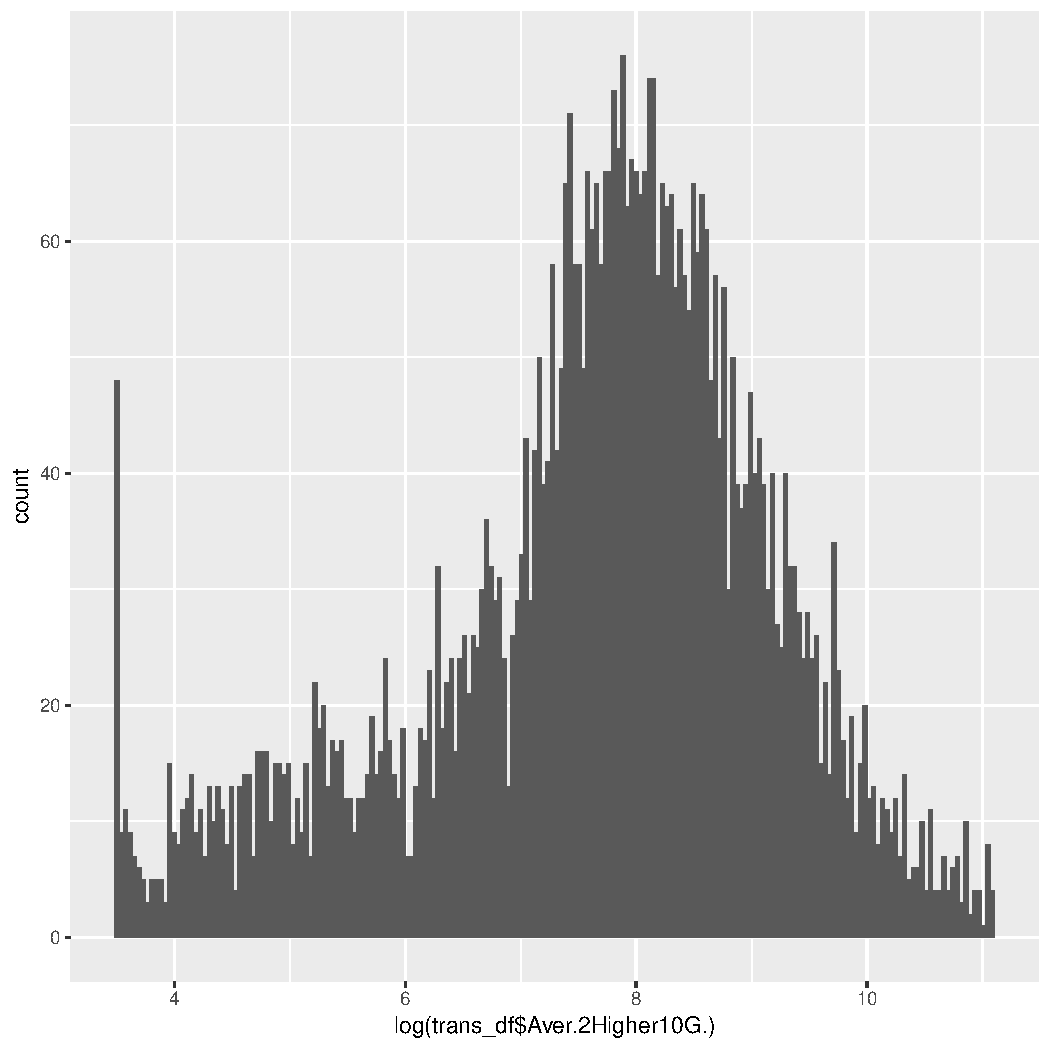
\includegraphics[width=\maxwidth]{figure/import_status_data-1} 

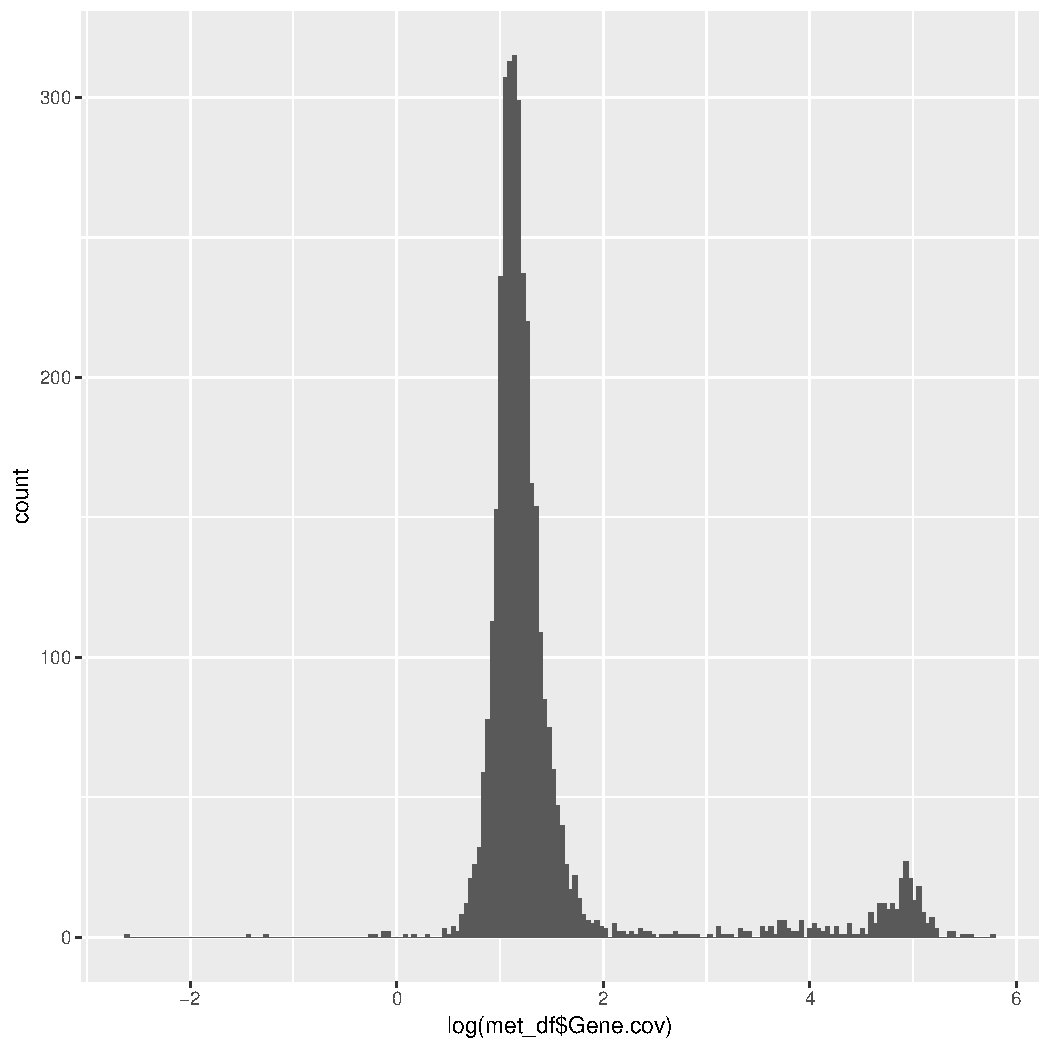
\includegraphics[width=\maxwidth]{figure/import_status_data-2} 
\begin{kframe}\begin{verbatim}
## 
## FALSE  TRUE 
##   214    74
## 
## FALSE  TRUE 
##    61    74
\end{verbatim}
\end{kframe}
\end{knitrout}

\section{Density Plots}
\subsection{log(Ac) All}
\begin{knitrout}
\definecolor{shadecolor}{rgb}{0.969, 0.969, 0.969}\color{fgcolor}
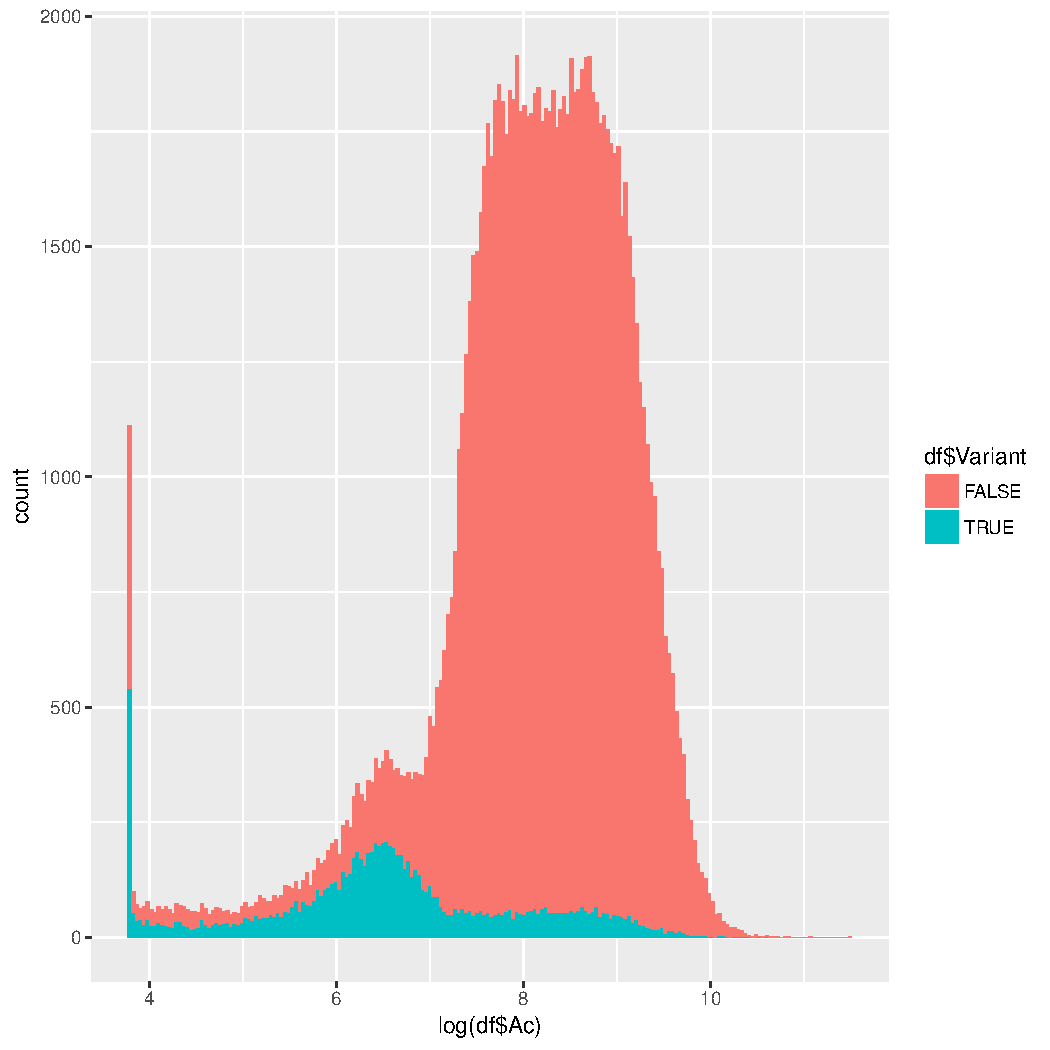
\includegraphics[width=1\linewidth]{figure/dens_all-1} 

\end{knitrout}
\clearpage
\subsection{log(Ac) 5'}
\begin{knitrout}
\definecolor{shadecolor}{rgb}{0.969, 0.969, 0.969}\color{fgcolor}
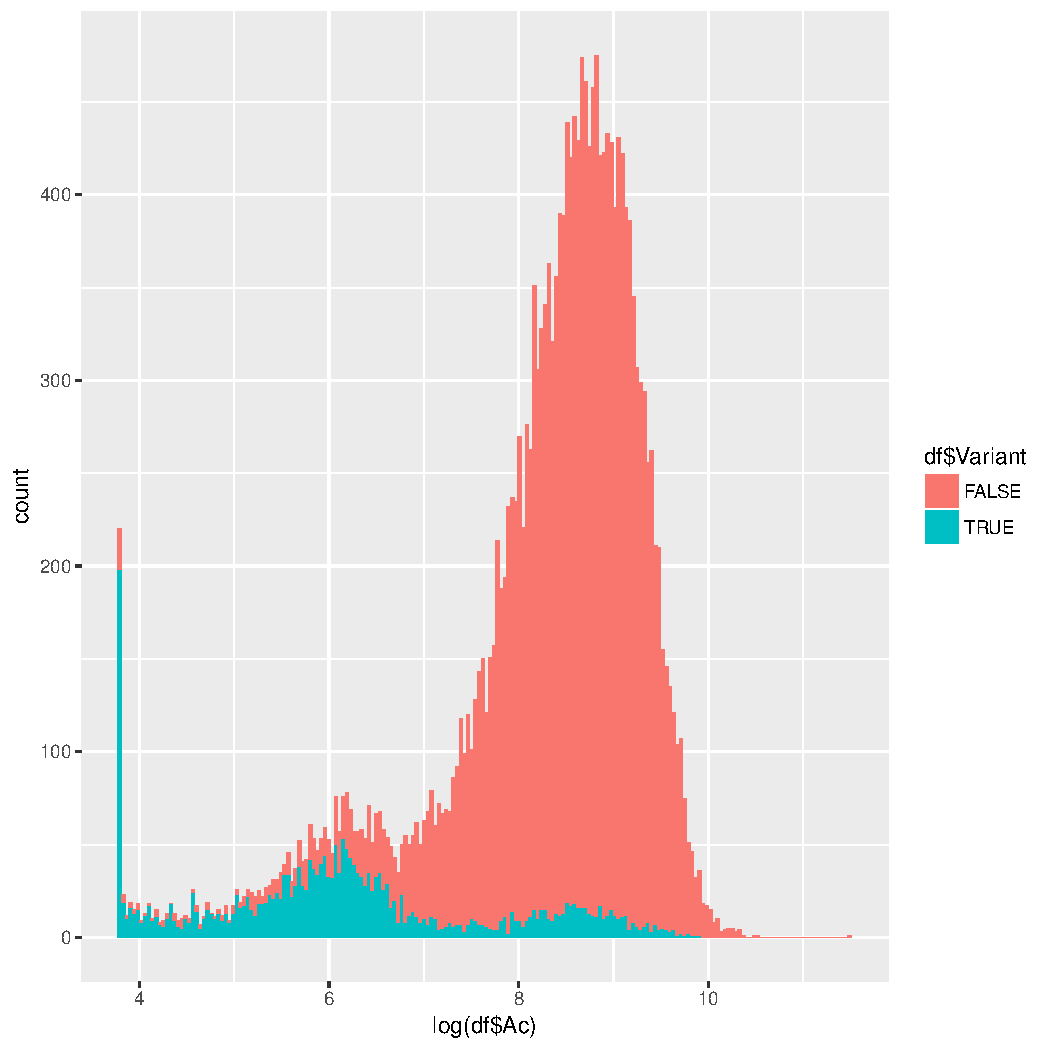
\includegraphics[width=1\linewidth]{figure/dens_5-1} 

\end{knitrout}
\clearpage
\subsection{log(Ac) 3'}
\begin{knitrout}
\definecolor{shadecolor}{rgb}{0.969, 0.969, 0.969}\color{fgcolor}
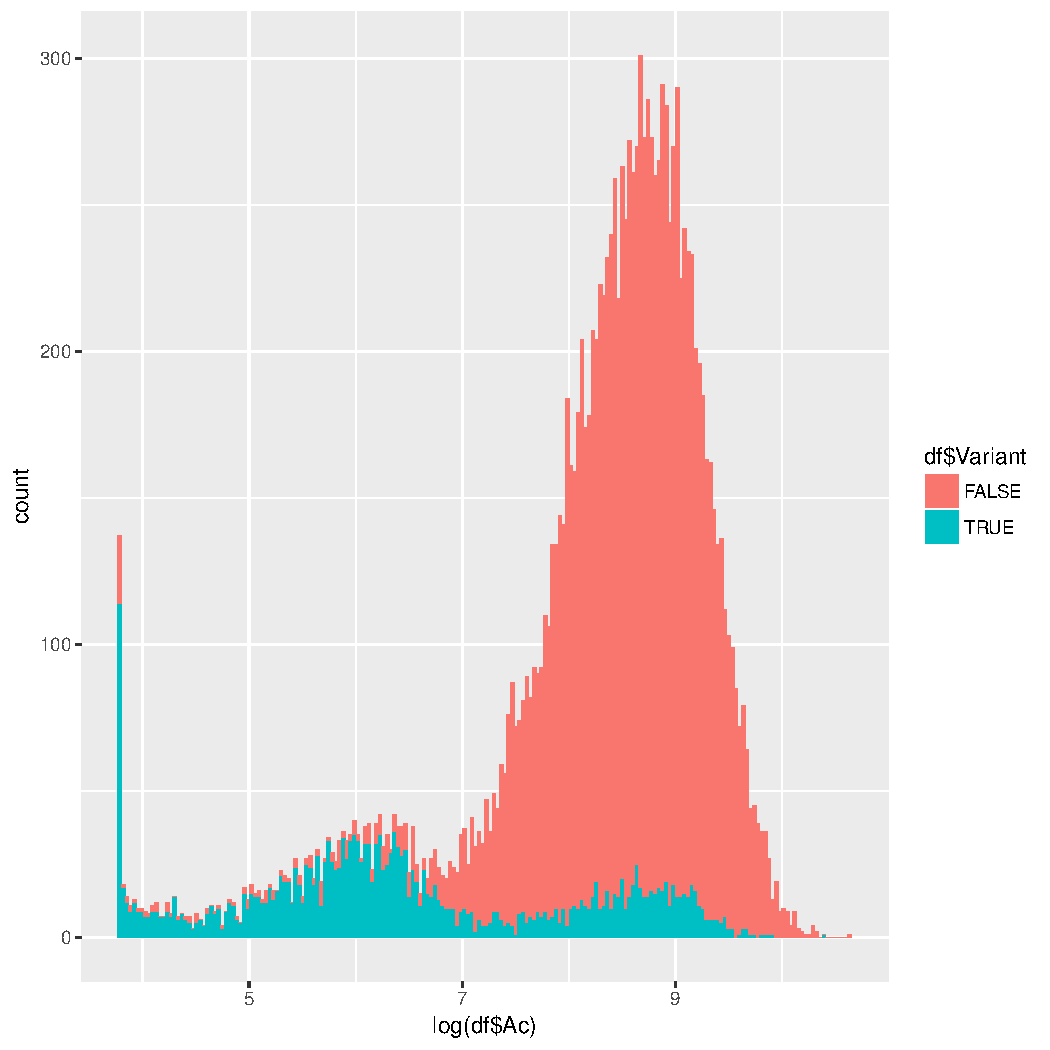
\includegraphics[width=1\linewidth]{figure/dens_3-1} 

\end{knitrout}
\clearpage
\subsection{log(Ac) ORF}
\begin{knitrout}
\definecolor{shadecolor}{rgb}{0.969, 0.969, 0.969}\color{fgcolor}
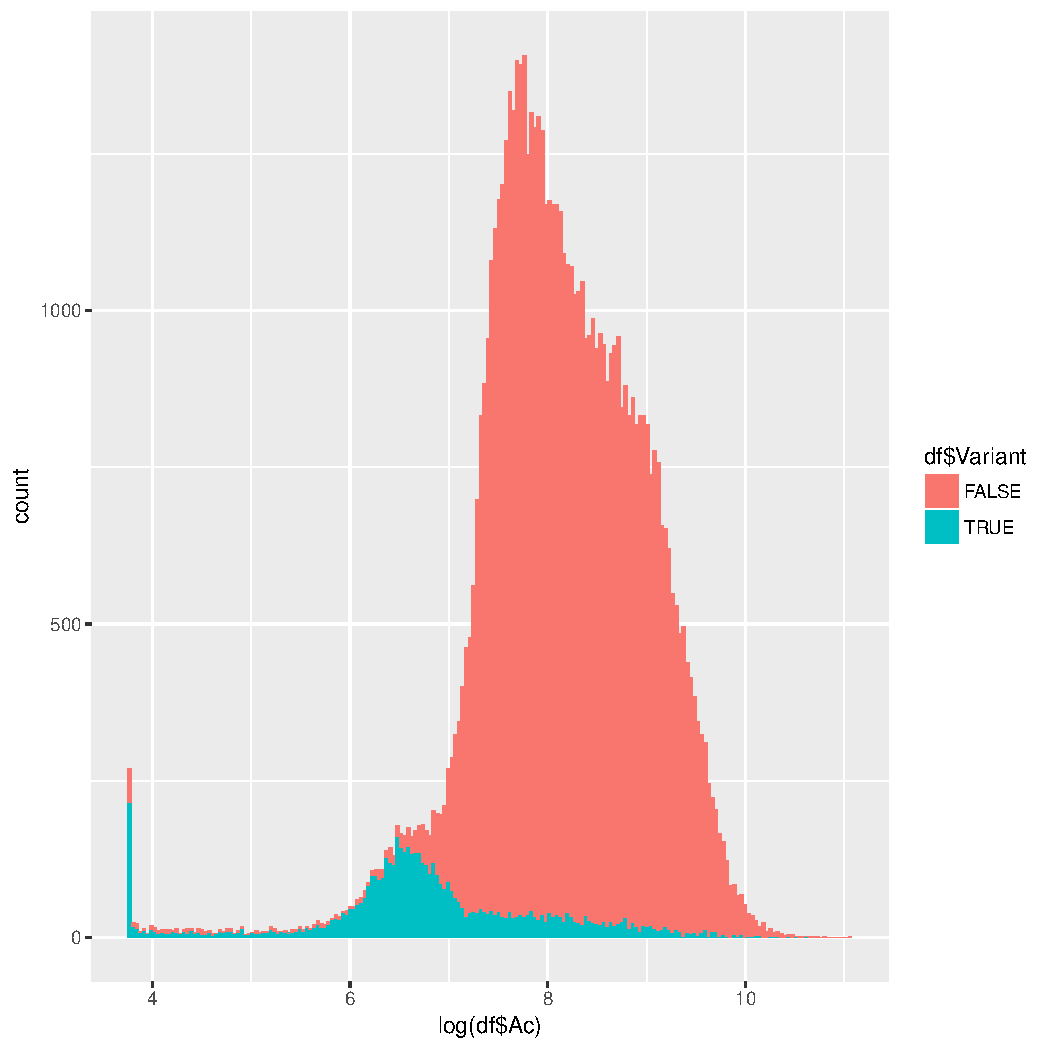
\includegraphics[width=1\linewidth]{figure/dens_ORF-1} 

\end{knitrout}
\clearpage
\subsection{log(Met) All}
\begin{knitrout}
\definecolor{shadecolor}{rgb}{0.969, 0.969, 0.969}\color{fgcolor}
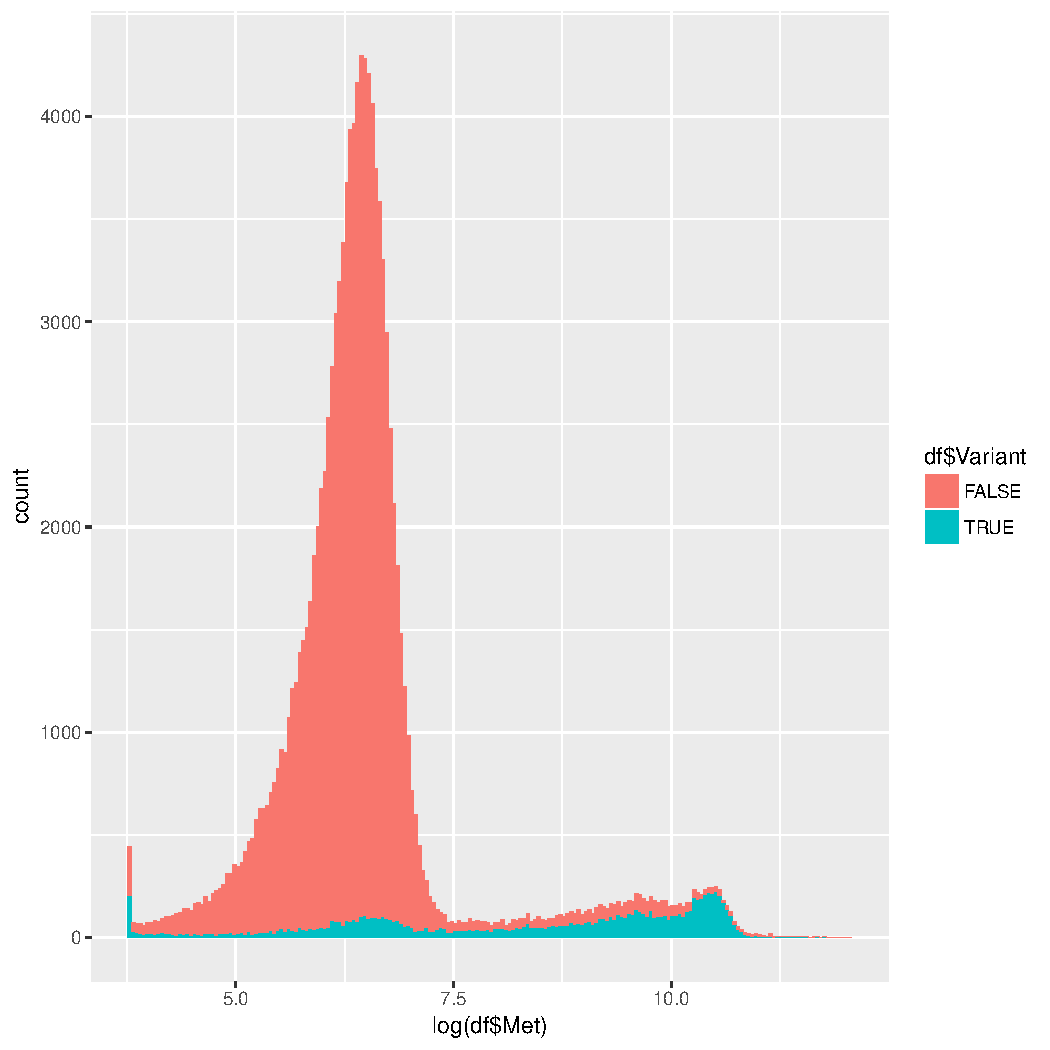
\includegraphics[width=1\linewidth]{figure/dens_all_met-1} 

\end{knitrout}
\clearpage
\subsection{log(Met) 5'}
\begin{knitrout}
\definecolor{shadecolor}{rgb}{0.969, 0.969, 0.969}\color{fgcolor}
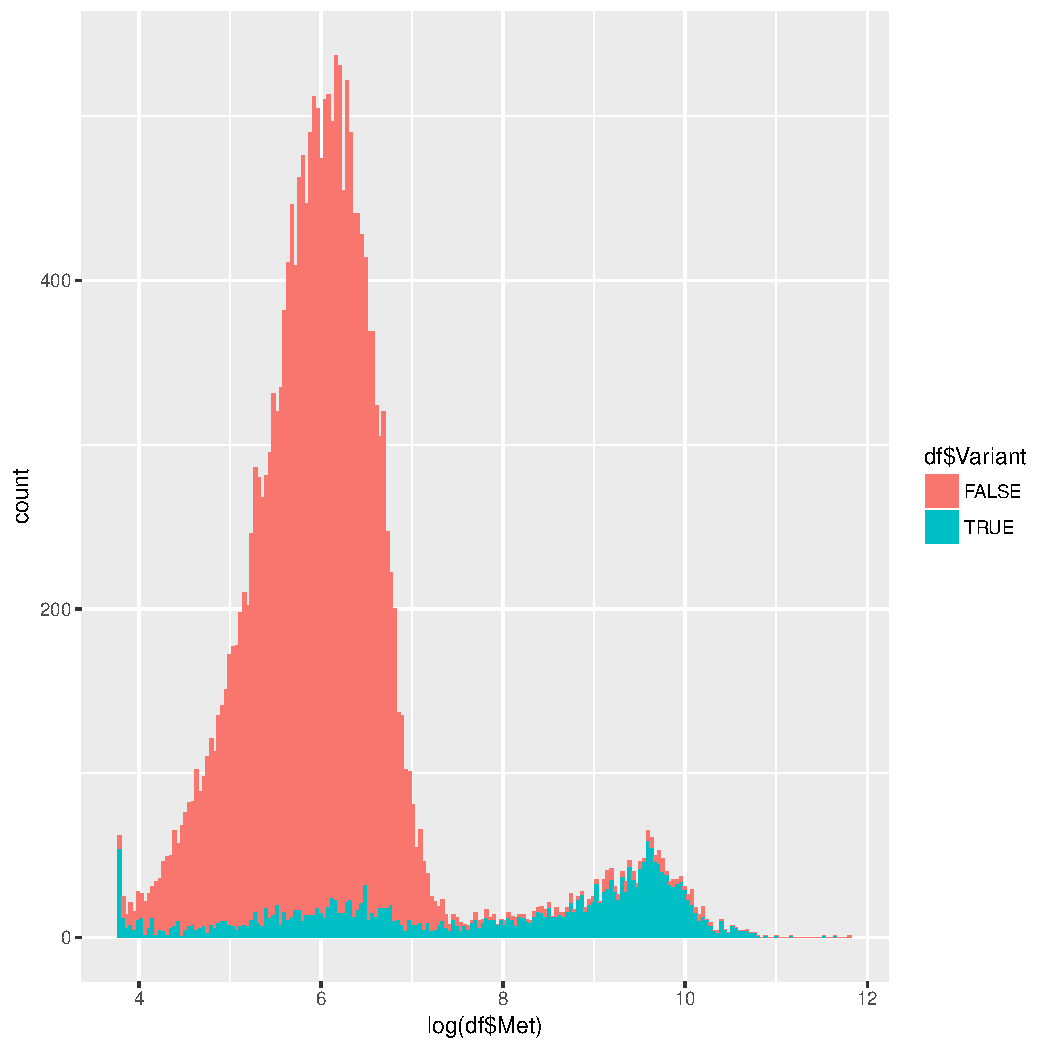
\includegraphics[width=1\linewidth]{figure/dens_5_met-1} 

\end{knitrout}
\clearpage
\subsection{log(Met) ORF}
\begin{knitrout}
\definecolor{shadecolor}{rgb}{0.969, 0.969, 0.969}\color{fgcolor}
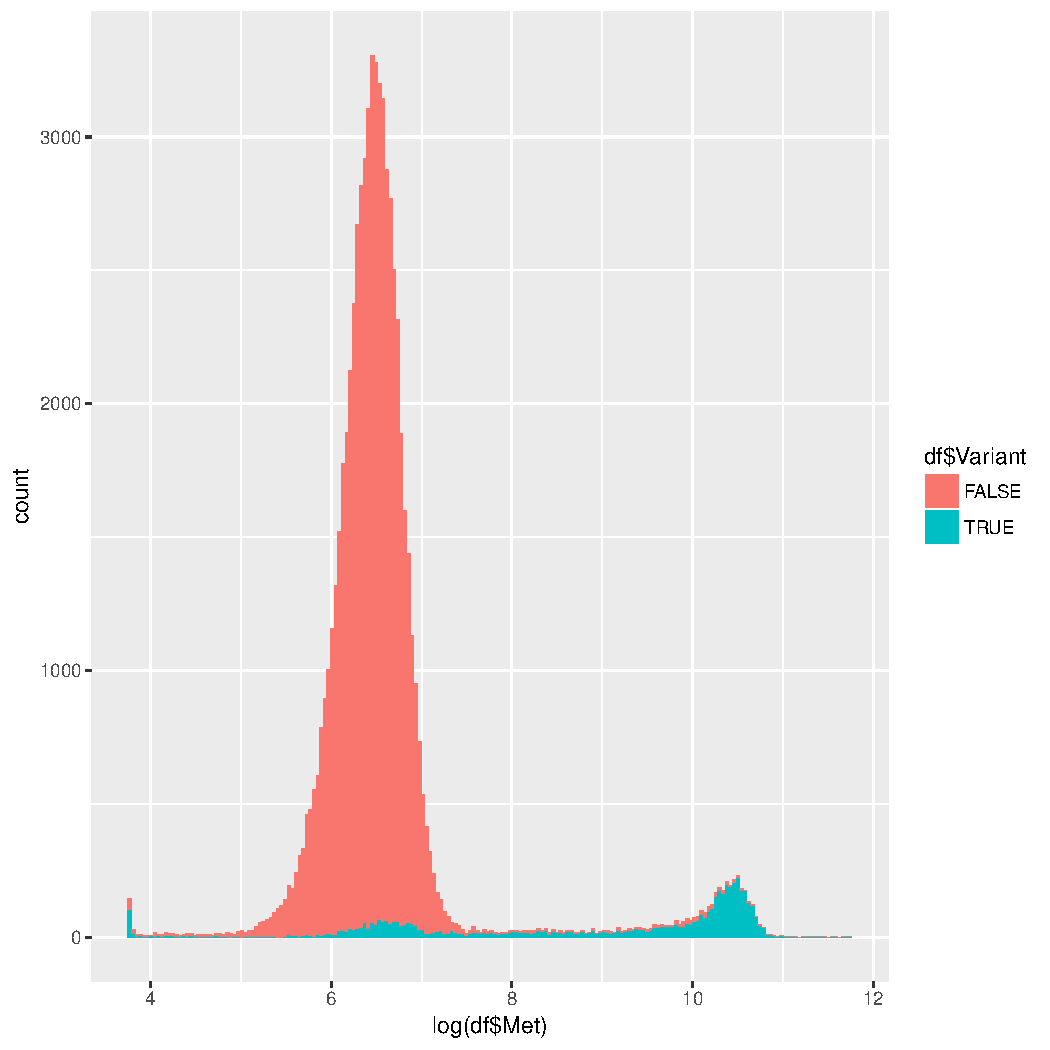
\includegraphics[width=1\linewidth]{figure/dens_ORF_met-1} 

\end{knitrout}
\clearpage
\subsection{log(Ac) 3'}
\begin{knitrout}
\definecolor{shadecolor}{rgb}{0.969, 0.969, 0.969}\color{fgcolor}
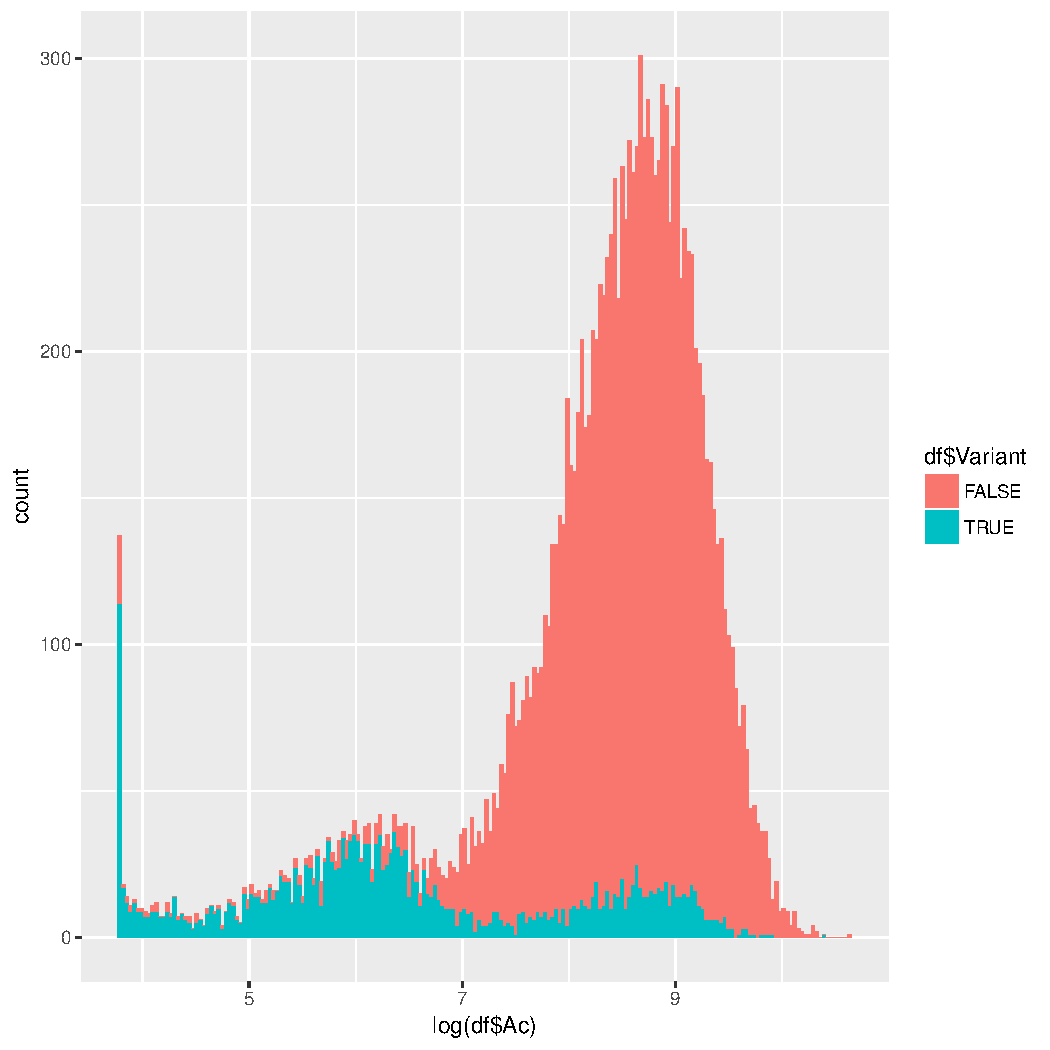
\includegraphics[width=1\linewidth]{figure/dens_3_met-1} 

\end{knitrout}

\begin{knitrout}
\definecolor{shadecolor}{rgb}{0.969, 0.969, 0.969}\color{fgcolor}\begin{kframe}
\begin{verbatim}
## 
##          Regular   Variant-Active Variant-Silenced 
##           105691             5530             5436
\end{verbatim}
\end{kframe}
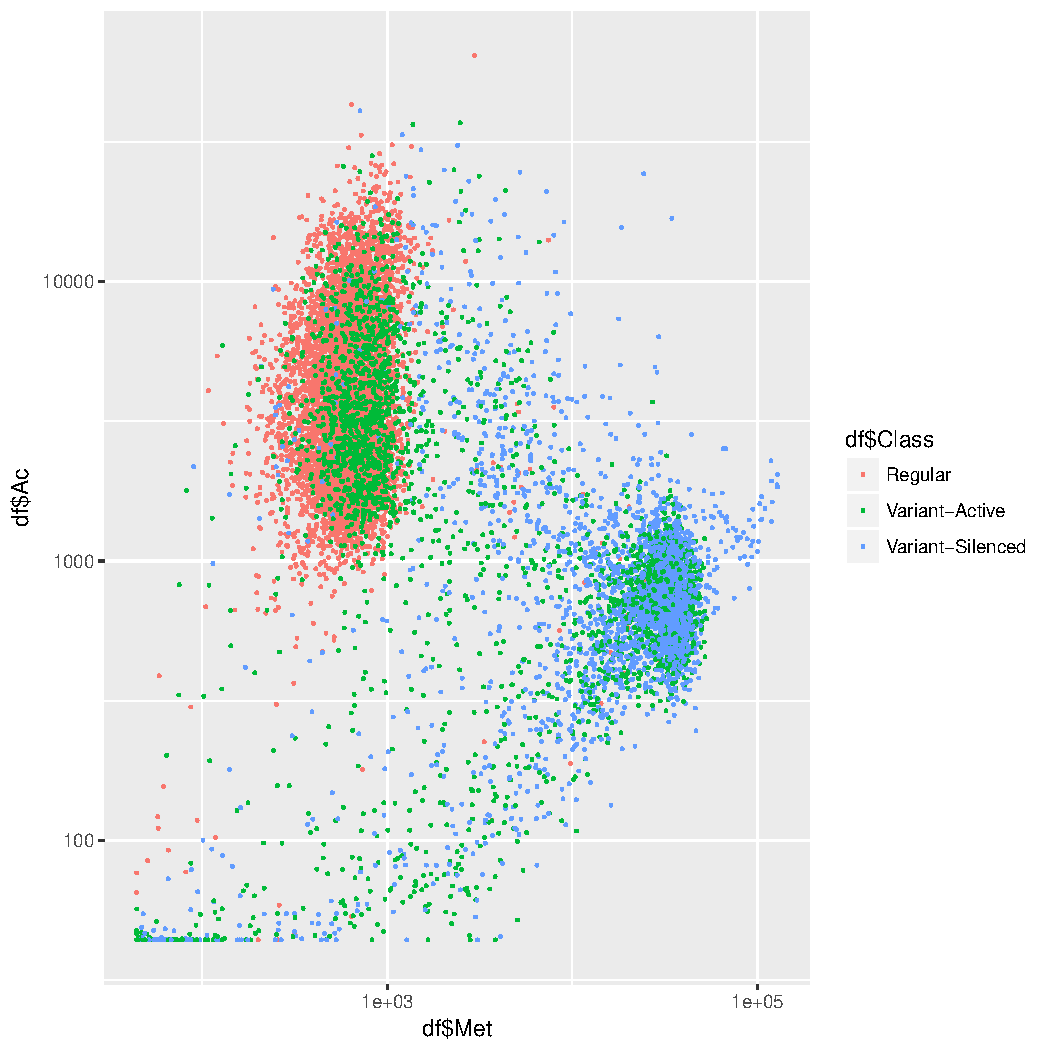
\includegraphics[width=1\linewidth]{figure/ac_met_log_status-1} 

\end{knitrout}

\begin{knitrout}
\definecolor{shadecolor}{rgb}{0.969, 0.969, 0.969}\color{fgcolor}\begin{kframe}
\begin{verbatim}
## 
##  FALSE   TRUE 
## 114212   2445
\end{verbatim}
\end{kframe}
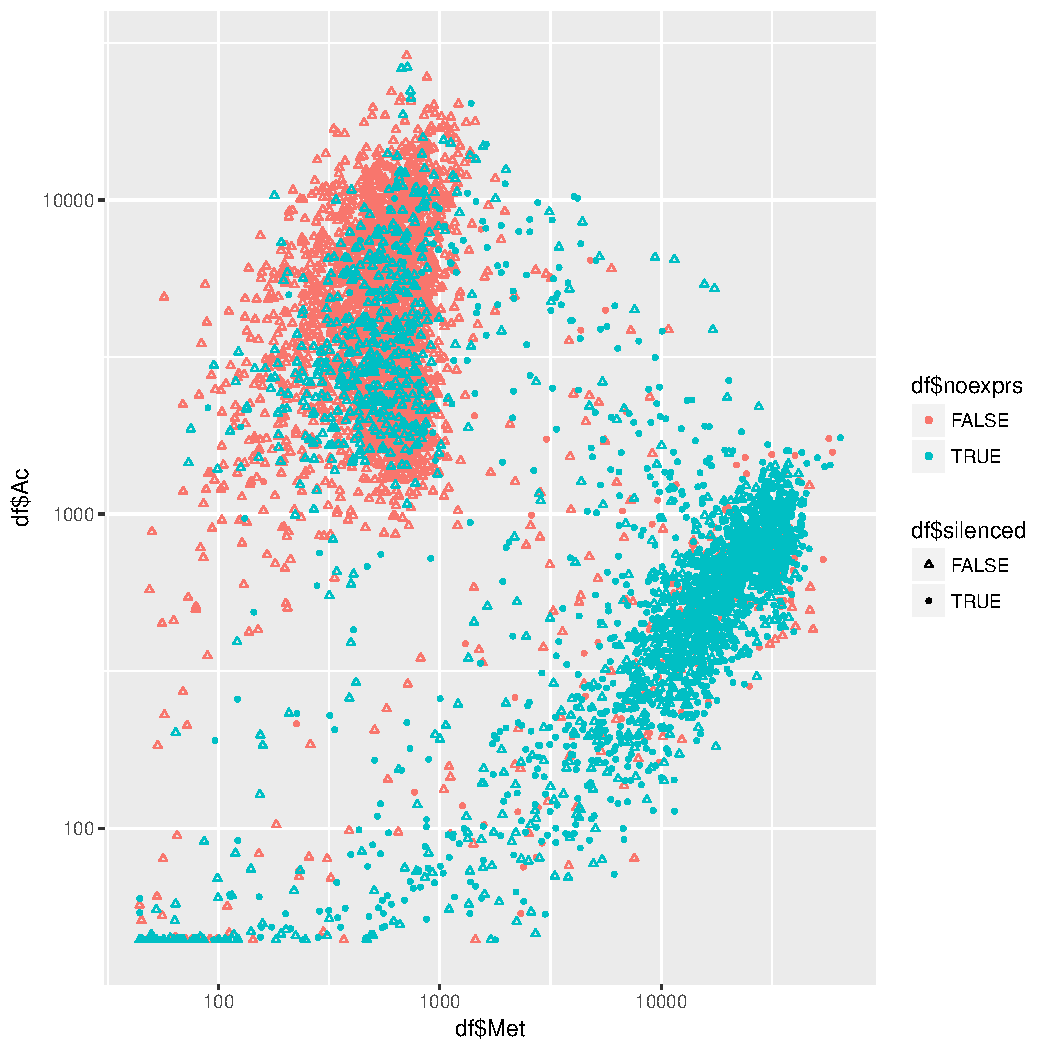
\includegraphics[width=1\linewidth]{figure/ac_met_log-1} 

\end{knitrout}

\begin{knitrout}
\definecolor{shadecolor}{rgb}{0.969, 0.969, 0.969}\color{fgcolor}\begin{kframe}
\begin{verbatim}
## 
##  FALSE   TRUE 
## 105691  10966
## Analysis of Deviance Table
## 
## Model 1: Variant ~ Ac + Met + Type + Start + Stop + silenced + noexprs
## Model 2: Variant ~ Ac + Met + Type + Start + Stop
##   Resid. Df Resid. Dev Df Deviance  Pr(>Chi)    
## 1      8477     5767.9                          
## 2      8479     6402.1 -2  -634.24 < 2.2e-16 ***
## ---
## Signif. codes:  0 '***' 0.001 '**' 0.01 '*' 0.05 '.' 0.1 ' ' 1
## 
## Call:
## glm(formula = Variant ~ Ac + Met + Type + Start + Stop + silenced + 
##     noexprs, family = binomial(link = "logit"), data = train_df)
## 
## Deviance Residuals: 
##     Min       1Q   Median       3Q      Max  
## -5.4070  -0.7659   0.0120   0.2261   2.8161  
## 
## Coefficients: (1 not defined because of singularities)
##                Estimate Std. Error z value Pr(>|z|)    
## (Intercept)   8.719e-01  9.888e-02   8.818  < 2e-16 ***
## Ac           -1.157e-04  9.326e-06 -12.409  < 2e-16 ***
## Met           2.663e-04  1.994e-05  13.352  < 2e-16 ***
## Type5prima   -4.064e-01  9.780e-02  -4.156 3.24e-05 ***
## TypeORF      -1.177e+00  8.561e-02 -13.750  < 2e-16 ***
## Typeother    -2.780e+01  1.516e+02  -0.183    0.854    
## Start        -2.517e-07  4.194e-08  -6.002 1.94e-09 ***
## Stop                 NA         NA      NA       NA    
## silencedTRUE  3.758e+00  2.672e-01  14.064  < 2e-16 ***
## noexprsTRUE   9.679e-01  2.330e-01   4.154 3.27e-05 ***
## ---
## Signif. codes:  0 '***' 0.001 '**' 0.01 '*' 0.05 '.' 0.1 ' ' 1
## 
## (Dispersion parameter for binomial family taken to be 1)
## 
##     Null deviance: 11127.3  on 8485  degrees of freedom
## Residual deviance:  5767.9  on 8477  degrees of freedom
## AIC: 5785.9
## 
## Number of Fisher Scoring iterations: 16
##        
##         FALSE TRUE
##   FALSE  2910  367
##   TRUE   1088 4480
## [1] "Accuracy 0.835500282645562"
## [1] "Accuracy of null model 0.502769926512154"
\end{verbatim}


{\ttfamily\noindent\itshape\color{messagecolor}{\#\# Loading required package: gplots}}

{\ttfamily\noindent\itshape\color{messagecolor}{\#\# \\\#\# Attaching package: 'gplots'}}

{\ttfamily\noindent\itshape\color{messagecolor}{\#\# The following object is masked from 'package:stats':\\\#\# \\\#\#\ \ \ \  lowess}}\end{kframe}
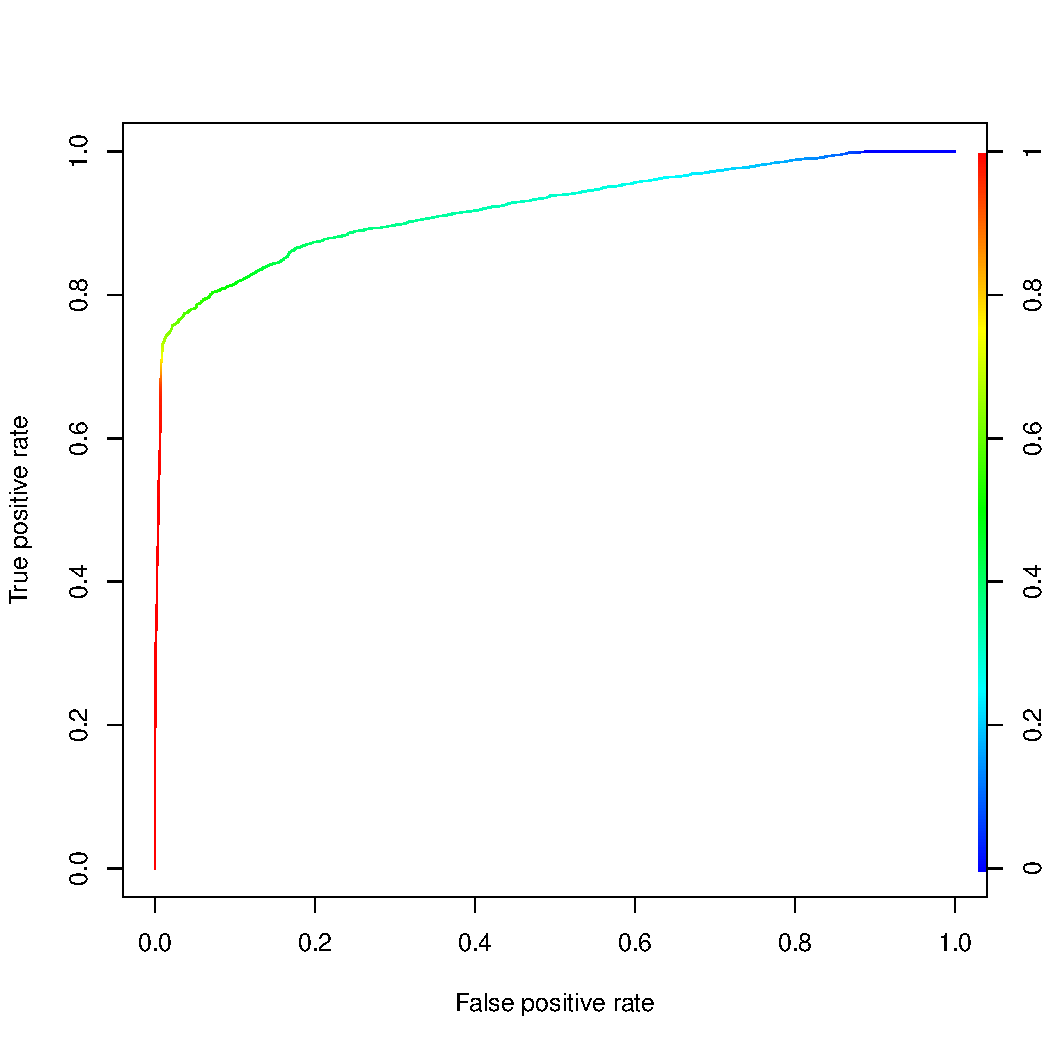
\includegraphics[width=\maxwidth]{figure/model-1} 
\begin{kframe}\begin{verbatim}
## 
## 3prima 5prima    ORF  other 
##    227    113     26      1
## 
## 3prima 5prima    ORF 
##    130    207    751
##           llh       llhNull            G2      McFadden          r2ML 
## -2883.9323527 -5563.6381013  5359.4114972     0.4816463     0.4682380 
##          r2CU 
##     0.6409677
\end{verbatim}
\end{kframe}
\end{knitrout}



\end{document}
